% !TEX root = ../main.tex

\label{appendix}

\begin{figure}
	\centering
	\begin{subfigure}{.5\textwidth}
		\centering
		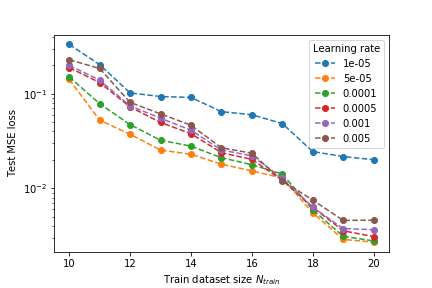
\includegraphics[width=1.1\linewidth]{lr_dim2_m3}
		\caption{2 dimensions}
	\end{subfigure}%
	\begin{subfigure}{.5\textwidth}
		\centering
		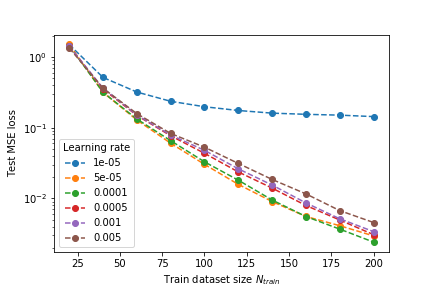
\includegraphics[width=1.1\linewidth]{lr_dim3_m3}
		\caption{3 dimensions}
	\end{subfigure}
	\caption{Comparison of learning rates for Model 3}
	\label{fig:comp_lr_m3}
\end{figure}

\begin{figure}[ht]
	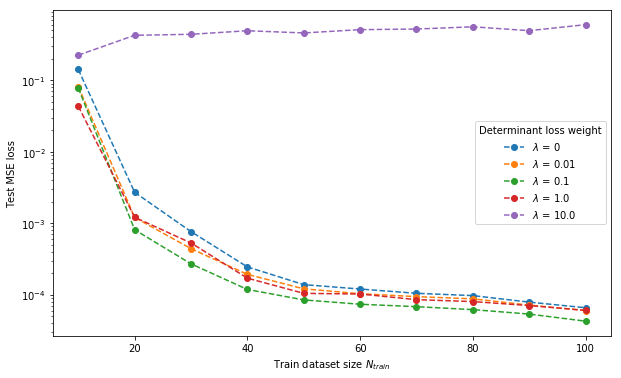
\includegraphics[width=\linewidth]{pnlty_det_large}
	\caption{Different weights $\lambda$ for $L_{DET}$ in 2D}
	\label{fig:pnlty_det_large}
\end{figure}


\clearpage
